\section*{Anexo I - Revisitando a linguagem de programação C}
\subsection*{Apontadores}
\

Para acessar o endereço de memória virtual de uma variável em C é utilizado o operador de referência $\&$, o endereço de memória é representado por 0x seguido de um número em base hexadecimal.

Um apontador é um tipo de variável cuja função é armazenar um endereço de memória virtual, se um apontador $p$ armazena o endereço de uma variável $x$ é possível então dizer que $p$ aponta para o endereço de $x$.

O processo de definir um apontador para um endereço significa que uma \textbf{referência} para o endereço é feita, já armazenar o identificador do endereço em uma variável é um processo de \textbf{dereferência}.

\begin{lstlisting}[language=C, frame=single]
    int x = 35;
    int* p = &x; //Referencia

    int d = *p; //Dereferencia
\end{lstlisting}

\subsection*{Aritmética de endereços}
\

A aritmética de endereços é importante para a alocação dinâmica. Na memória virtual, os endereços dos elementos de um vetor são armazenados de modo sequencial. Ao declarar um vetor $V$, sendo $i$ uma constante $i=0, 1 ...$ \textit{tamanho do vetor} $-1$, acessar $V[i]$ é idêntico a acessar $*(V+i)$.

\begin{lstlisting}[language=C, frame=single]
    int* V; 
    V = malloc (10*sizeof(int));
    //V[i]=*(V+i)
\end{lstlisting}

\newpage

\begin{figure}
  \centering
  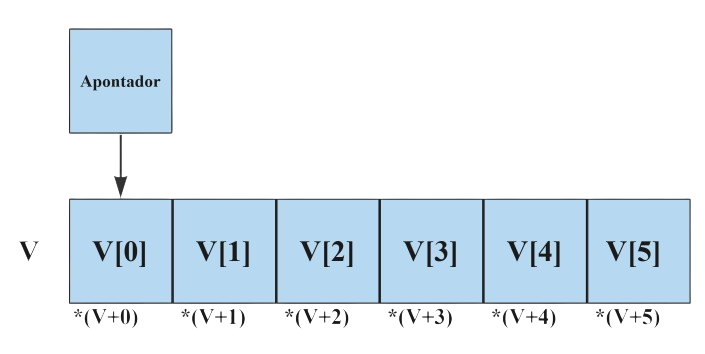
\includegraphics[width=0.7\linewidth]{img/aritmeticaenderecos.png}
    \caption{Representação da aritmética de endereços}
    \label{aritimeticaenderecos}
\end{figure}

Para o caso de matrizes $M[i][j]=*(*(M+i)+j)$.

\subsection*{Alocação dinâmica}
\

Diferentemente da alocação estática, a alocação dinâmica permite que a memória utilizada durante a execução do programa seja administrada através de funções.

A função \texttt{malloc} é utilizada para alocar um bloco de memória na \textit{heap} onde o argumento é o número de \textit{bytes} alocados, \texttt{sizeof} é um operador que indica quantos \textit{bytes} tem o parâmetro.

\begin{center}
\texttt{void* malloc(size\_t size)}
\end{center}

A função \texttt{calloc} aloca o bloco de memória solicitado retornando um apontador para ele, a diferença entre as funções \texttt{malloc} e \texttt{calloc} é que na segunda a memória alocada é definida para zero.

\begin{center}
\texttt{void* calloc(size\_t nitems, size\_t size)}
\end{center}

Para redimensionar a memória já alocada é utilizada a função \texttt{realloc}, essa função traz uma dinamicidade maior para a memória. Os argumentos necessários são um apontador para o bloco previamente alocado e o novo tamanho.

\begin{center}
\texttt{void* realloc(void* ptr, size\_t size)}
\end{center}

As variáveis armazenadas estaticamente são excluídas no final da função correspondente, no entanto, para a memória dinamicamente alocada é necessário o uso da função \texttt{free} é necessário. Essa função desaloca um bloco de memória previamente alocado.

\begin{center}
\texttt{void free(void* ptr)}
\end{center}

\subsection*{Vetores e matrizes dinâmicos}
\

É possível, através de apontadores alocar vetores e matrizes. Uma matriz basicamente pode ser interpretada como apontadores duplos, os códigos abaixo demonstram como fazer essa alocação de memória e como libera-la com \texttt{free}.

\begin{lstlisting}[language=C, frame=single]
//alocando vetor dinamico
int* V; 

V = malloc (n*sizeof(int));

for(int i = 0; i < n; i++)
{
    //procedimentos
}

//desalocando vetor dinamico
free (V);
\end{lstlisting}

\begin{lstlisting}[language=C, frame=single]
//alocando matriz dinamica
int **M; 
M = malloc (m*sizeof(int*));

for (int i = 0; i < linhas; i++)
{
   *(M+i) = malloc(colunas*sizeof(int));
}

//desalocando matriz dinamica
for (int i = 0; i < linhas; i++) {
    free(*(M+i));
}

\end{lstlisting}